\section{Experimental setup}
In this section, the scheme of runtime partial evaluation is presented as well as the evaluation configuration.

\subsection{Runtime partial evaluation}

\begin{figure}
    \centering
    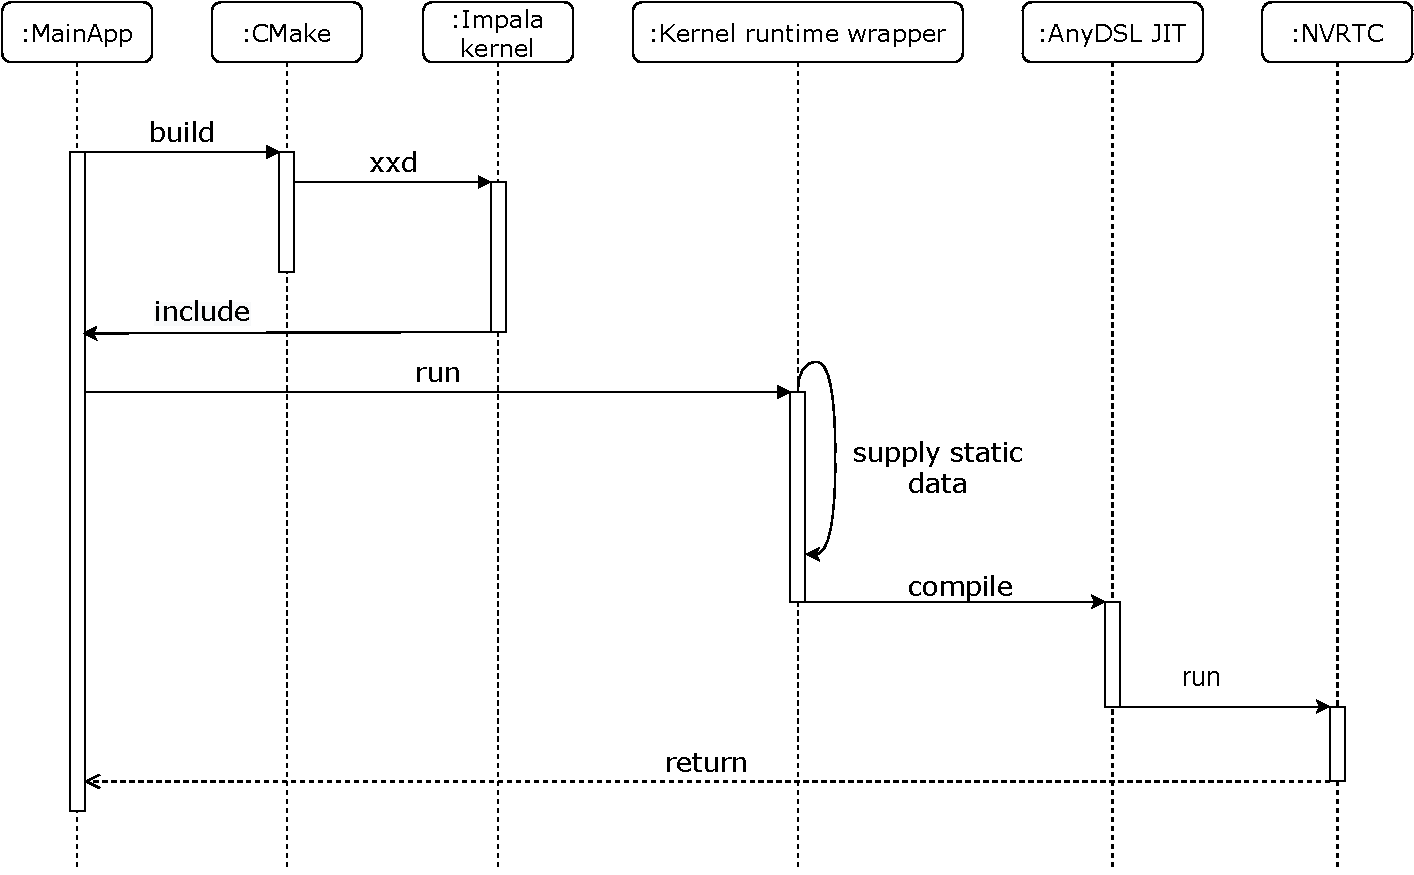
\includegraphics[width=\linewidth]{figures/SeqDiagram.pdf}
    \caption{Runtime partial evaluation diagram}
    \label{fig:seq_pe}
\end{figure}

In practice, it is infeasible to compile a new kernel for each static input 
value, which is often known in runtime. Thus the partial evaluation of the 
kernel should be performed in runtime as well as the kernel compilation to 
a specific GPU target.
Each specialized benchmark scenario corresponds to the sequence in 
figure~\ref{fig:seq_pe}. The device kernel in Impala is included in the 
target application using \lstinline{xxd} tool during the compilation. 
When static data becomes known at runtime, the kernel wrapper is constructed, 
that supplies the static data to the included kernel, 
creating partially applied kernel. Then AnyDSL JIT compiler is invoked, 
which specializes the kernel according to the annotations provided, 
and static arguments supplied, generating CUDA C code, which is then passed 
to NVRTC\,\footnote{\url{https://docs.nvidia.com/cuda/nvrtc/index.html} (last accessed date: 30.05.2020)} 
and got eventually compiled to GPU assembly and invoked.

The evaluation aim is to show whether a device kernel could benefit from data 
embedding performed by partial evaluation and possible reduction of 
static computations. For the data to be embedded, the accesses should 
be static, which is a standard scenario for constant memory to be used to store such data, 
thus constant memory is a baseline in several scenarios. 
Further, only the execution time of a device kernel should be measured, 
since, for example, overhead for partial evaluation and JIT compilation 
for a device could be hidden by GPU data transferring or other workarounds.

Since NVRTC is internal to AnyDSL framework, 
the benchmarking results could be obtained via 
nvprof\,\footnote{\url{https://docs.nvidia.com/cuda/profiler-users-guide/index.html} \\ (last accessed date: 30.05.2020)} 
or by utilizing a specially recompiled version of the framework 
runtime with CUDA events. 
The latter option is used since it allows to perform warm-up runs of the kernel 
to make the benchmarking more reliable. The whole system is implemented in C++ and Python, 
and enclosed into a Docker container with the datasets indexed in Git LFS\footnote{\url{https://git-lfs.github.com/} (last accessed date: 30.05.2020)}
 for benchmarks to be easily built and run on any system with NVIDIA GPU\,\footnote{\url{https://github.com/Tiltedprogrammer/spec} (last accessed date: 30.05.2020)}. 
 The following GPGPU scenarios have been implemented, which are fit under the described in~\ref{PEsurvey} pipeline.
\begin{itemize}
    \item Na\'ive single substring matching.
    \item Na\'ive multiple substring matching.
    \item Aho--Corasick matching.
    \item 2-D convolution filter.
\end{itemize}
The following system has been used to run the benchmarks: 
Ubuntu 18.04 with CUDA Toolkit 10.2. hosted in Google Cloud 
bundled with 4 cores of Intel Xeon and NVIDIA Tesla T4 GPU.
